% Provenance (never printed): old terminale S material on absolute dating (the
% decay law recalled, the closed system, the rubidium-strontium isochron) and on
% the history of the age of the Earth (cooling, salt, sediments, then radioactivity,
% meteorites and 4.55 billion years). Owner (Sync 0/1): closed system, isochron,
% age of the Earth (as a defined notion). The decay law, the half-life and the
% dating equation are the physics books' (recalled); relative dating, absolute
% age, superposition, cross-cutting relationships and the eras are Book 1 g7's
% (recalled); the oldest zircons and the Acasta gneiss are g12.01's (quoted).
% Varden Hills granite 310 Ma and schist 480 Ma from figdata/shared/region.py;
% their isotope ratios are exercise data (figdata/grade-12/isochrons.py).
\chapter{Radiometrische datering en de ouderdom van de Aarde}\label{ch:g12:age-of-the-earth}

In 1862 berekende de natuurkundige William Thomson, later Lord Kelvin, hoe oud de
Aarde is uit de manier waarop ze afkoelt. Hij nam aan dat ze gesmolten was ontstaan en
sindsdien haar warmte verloor, en vroeg hoe lang het zou duren tot de
temperatuurgradiënt dicht bij het oppervlak tot zijn huidige waarde was gedaald. Zijn
antwoord was 96 miljoen jaar, ergens tussen 20 en 400
miljoen; in 1897 had hij het vernauwd tot tussen 20 en 40 miljoen.
Geologen vonden dat veel te kort voor de geschiedenis die ze in de gesteenten lazen.
Het antwoord kwam van de radioactiviteit, die Kelvin niet kende.
% ledger: holmes13:estimates, england:kelvin (Book 3 row)

\begin{omfigure}
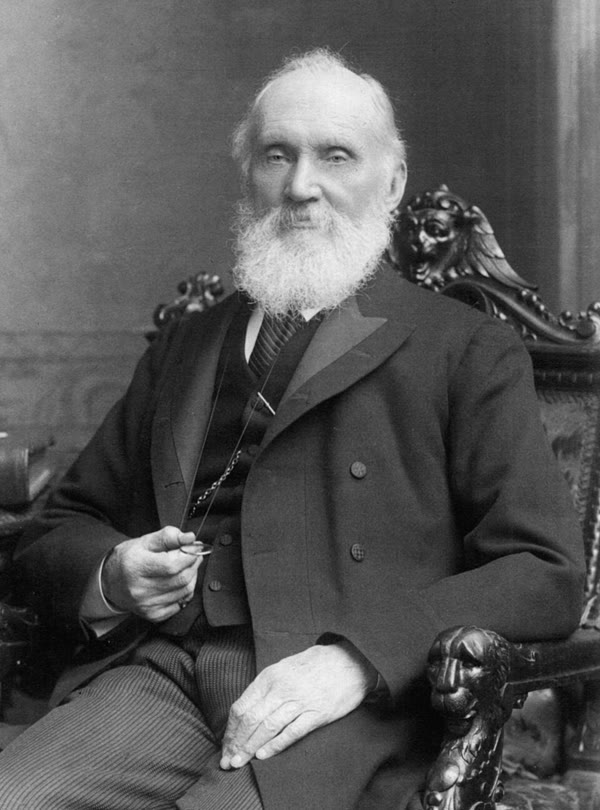
\includegraphics[height=5.2cm]{images/book2/g12-kelvin-1906.jpg}

{\small William Thomson, Lord Kelvin, in 1906. Foto Russell and Sons,
Londen (Smithsonian Institution Libraries, geen bekende auteursrechtelijke beperkingen).}
\end{omfigure}
% ledger: photo:g12-kelvin

\begin{recall}
Relatieve datering zet gesteenten en gebeurtenissen op volgorde; een absolute ouderdom is een aantal
jaren (Boek 1, jaar 7). Een radioactieve isotoop, de moederisotoop, vervalt willekeurig tot een
dochterisotoop: het aantal $N$ moederatomen dat overblijft, daalt als
$N = N_0\,e^{-\lambda t}$, waarbij $\lambda$ de vervalconstante is, en halveert
elke halveringstijd $T = \ln 2/\lambda$ (de natuurkundeboeken). De oudste bekende
mineralen, zirkoonkorrels uit West-Australië, zijn 4.4 miljard jaar oud
(\cref{ch:g12:continental-crust}). De Aarde verliest ook warmte die radioactiviteit
blijft aanmaken, en haar mantel convecteert (\cref{ch:g12:internal-heat}).
\end{recall}
% ledger: wilde01:zircon

\section{Een geschiedenis van schattingen}

Vóór de radioactiviteit berustte elke schatting van de \omterm{def:g12:age-of-the-earth:age}{ouderdom van de Aarde} op een proces
waarvan men de snelheid bekend veronderstelde.

\begin{center}
\small
\begin{tabular}{|p{0.19\linewidth}|p{0.42\linewidth}|p{0.25\linewidth}|}
\hline
wie, wanneer & methode en wat ze aanneemt & schatting \\
\hline
Phillips, 1860 & dikte van de sedimentaire lagen gedeeld door een afzettingssnelheid; neemt een constante snelheid aan & 38 tot 96 miljoen jaar \\
Kelvin, 1862 & afkoeling van een gesmolten Aarde door geleiding alleen, zonder warmtebron binnenin & 20 tot 400 miljoen jaar \\
G.\,H.~Darwin & tijd sinds de Maan zich van de Aarde afscheidde, uit het vertragen van hun bewegingen door de getijden & minstens 56 miljoen jaar \\
Joly, 1899 & zout dat rivieren naar zee voeren, gedeeld door de jaarlijkse aanvoer; neemt een constante aanvoer aan en geen zout dat wordt verwijderd & 80 tot 100 miljoen jaar \\
\hline
\end{tabular}
\end{center}
% ledger: holmes13:estimates

\begin{history}[De ontbrekende warmte van Kelvin]
In 1903 toonden Pierre Curie en Albert Laborde aan dat radium warmte afgeeft,
en verscheidene wetenschappers betoogden al snel dat deze warmte de conclusie van Kelvin
omverwierp. Een jaar later herinnerde Ernest Rutherford, die een lezing gaf met Kelvin in
het publiek, hem eraan dat hij de \omterm{def:g12:age-of-the-earth:age}{ouderdom van de Aarde} had begrensd
``op voorwaarde dat er geen nieuwe warmtebron werd ontdekt''. Radioactiviteit leek
die bron te zijn. Toch was dat niet Kelvins voornaamste fout: wat het afkoelen van de Aarde het meest verlengt,
is \omterm{def:g12:internal-heat:convection}{mantelconvectie}, die de bovenmantel heet houdt en de gradiënt in
de korst veel langer hoog dan geleiding alleen zou doen.
\end{history}
% ledger: england:kelvin (Book 3 row)

De radioactiviteit gaf ook een klok. In 1907 toonde Bertram Boltwood aan dat
uraniummineralen van dezelfde ouderdom dezelfde hoeveelheid lood per gram
uranium bevatten: het lood wordt door het uranium gemaakt. In 1913 kon Arthur Holmes
schrijven dat de oudste gedateerde gesteenten \num{1600} miljoen jaar oud waren, en in
1927 legde hij de \omterm{def:g12:age-of-the-earth:age}{ouderdom van de Aarde} tussen 1.6 en 3.0 miljard jaar. In 1956 mat Clair
Patterson 4.55 miljard jaar. De waarde van vandaag is 4.54 miljard jaar,
tot op één procent nauwkeurig.
% ledger: holmes13:estimates, holmes27:age, patterson56:table, usgs:age-earth (Book 1 row)

\begin{omfigure}
\begin{tikzpicture}
\begin{axis}[omrecord, width=0.78\linewidth, height=6.2cm, ymode=log, xmin=1840, xmax=2040,
  ymin=1e7, ymax=2e10, xlabel={jaar van de schatting}, ylabel={geschatte ouderdom van de Aarde (jaar)},
  xtick={1850,1875,...,2025}, x tick label style={/pgf/number format/.cd, set thousands separator={}},
  ytick={1e7,1e8,1e9,1e10}, ymajorgrids=true, xmajorgrids=false]
% computed in figdata/grade-12/isochrons.py; ledger: holmes13:estimates, holmes27:age, patterson56:table, usgs:age-earth (Book 1 row)
\addplot[omDef, only marks, mark=*, mark size=1.8pt, error bars/.cd, y dir=both, y explicit]
  table[x=year, y=mid, y error minus expr=\thisrow{mid}-\thisrow{lo}, y error plus expr=\thisrow{hi}-\thisrow{mid}]
  {figdata/out/grade-12-isochrons-history.dat};
\addplot[omThm, densely dashed, domain=1840:2040, samples=2] {4.54e9};
\coordinate (k62) at (axis cs:1862,2.4e8);
\coordinate (k97) at (axis cs:1897,2.8e7);
\coordinate (jol) at (axis cs:1899,1e8);
\coordinate (h11) at (axis cs:1919,1.3e9);
\coordinate (pat) at (axis cs:1956,4.55e9);
\coordinate (now) at (axis cs:1845,4.54e9);
\end{axis}
\node[font=\scriptsize, anchor=west] at ([xshift=4pt]k62) {Kelvin 1862};
\node[font=\scriptsize, anchor=east] at ([xshift=-4pt]k97) {Kelvin 1897};
\node[font=\scriptsize, anchor=west] at ([xshift=4pt]jol) {Joly};
\node[font=\scriptsize, anchor=north] at (h11) {Holmes};
\node[font=\scriptsize, anchor=north west] at ([xshift=2pt, yshift=-3pt]pat) {Patterson};
\node[font=\scriptsize, text=omThm, anchor=south west] at (now) {vandaag, 4.54 miljard jaar};
\end{tikzpicture}

{\small Schattingen van de \omterm{def:g12:age-of-the-earth:age}{ouderdom van de Aarde} tegen het jaar waarin ze werden gemaakt, op
een logaritmische schaal; de staafjes bestrijken het bereik dat elke auteur gaf. Het punt van Holmes
uit 1913 is de ouderdom van de oudste gesteenten die toen waren gedateerd, een minimum. Bronnen: Holmes
(1913, 1927); Patterson (1956); U.S. Geological Survey.}
\end{omfigure}

\section{Een radioactieve klok}

Een radioactieve klok werkt alleen als er niets aan is toegevoegd of van is
weggenomen sinds hij begon te lopen.

\begin{definition}[Gesloten systeem]\label{def:g12:age-of-the-earth:closed-system}
Een gesteente of een mineraal is een \emph{gesloten systeem}\index{gesloten systeem} voor een
moederisotoop en zijn dochter als er, sinds het moment dat zijn klok begon te lopen,
geen atoom van de moeder of van de dochter in of uit is gegaan, anders dan
door het verval van de moeder tot de dochter.
\end{definition}
% ledger: tulane:radiometric

Voor een mineraal begint de klok te lopen wanneer het uit een magma kristalliseert, of
preciezer, wanneer het genoeg is afgekoeld opdat de atomen er niet meer in en uit
bewegen. Verhitting, een hete
vloeistof of verwering kan het systeem weer openen, en de ouderdom die dan wordt gemeten, is
fout, of dateert die latere gebeurtenis.
% ledger: tulane:radiometric

Wie de dochteratomen in een \omterm{def:g12:age-of-the-earth:closed-system}{gesloten systeem} telt, krijgt de ouderdom, op voorwaarde dat men
weet hoeveel er bij het begin waren. Meestal weet men dat niet. Rubidium-87
vervalt tot strontium-87, maar elk mineraal nam bij zijn ontstaan ook wat strontium-87
op. De isochroonmethode omzeilt dit door verscheidene
mineralen van één gesteente te meten.

\section{De isochroon}

Strontium heeft een isotoop, strontium-86, die stabiel is en door geen enkel
verval wordt gemaakt: in een \omterm{def:g12:age-of-the-earth:closed-system}{gesloten systeem} blijft zijn aantal gelijk, en hij dient als
maatstaf. De isotopenverhoudingen $^{87}\mathrm{Sr}/^{86}\mathrm{Sr}$ en
$^{87}\mathrm{Rb}/^{86}\mathrm{Sr}$ zijn wat een massaspectrometer meet.

\begin{theorem}[De isochroonvergelijking]\label{thm:g12:age-of-the-earth:isochron}
In een mineraal dat gedurende een tijd $t$ een \omterm{def:g12:age-of-the-earth:closed-system}{gesloten systeem} is geweest, geldt
\[
  \left(\frac{^{87}\mathrm{Sr}}{^{86}\mathrm{Sr}}\right)_{\text{nu}}
  = \left(\frac{^{87}\mathrm{Sr}}{^{86}\mathrm{Sr}}\right)_{0}
  + \left(\frac{^{87}\mathrm{Rb}}{^{86}\mathrm{Sr}}\right)_{\text{nu}}
  \left(e^{\lambda t} - 1\right),
\]
waarbij de index 0 de waarde aangeeft toen de klok begon te lopen en $\lambda$
de vervalconstante van rubidium-87 is.
\end{theorem}

\begin{proof}
Laat $P$ het aantal rubidium-87-atomen nu zijn en $P_0$ toen de klok
begon te lopen. Volgens de vervalwet is $P = P_0\,e^{-\lambda t}$, dus $P_0 = P\,e^{\lambda t}$,
en het aantal atomen dat is vervallen, is $P_0 - P = P\,(e^{\lambda t}-1)$.
In een \omterm{def:g12:age-of-the-earth:closed-system}{gesloten systeem} is elk ervan één atoom strontium-87 geworden, dat
wordt toegevoegd aan de $D_0$ atomen die er bij het begin waren: $D = D_0 + P\,(e^{\lambda
t}-1)$. Delen door het aantal strontium-86-atomen, dat niet is veranderd,
geeft de vergelijking.
\end{proof}
% ledger: tulane:radiometric

De mineralen van een graniet kristalliseerden uit één magma, dus begonnen ze allemaal
met dezelfde verhouding $(^{87}\mathrm{Sr}/^{86}\mathrm{Sr})_0$. Maar ze namen
heel verschillende hoeveelheden rubidium op. Ze delen allemaal dezelfde $t$ en dezelfde beginverhouding, dus
zegt de vergelijking dat hun punten op één rechte liggen.

\begin{definition}[Isochroon]\label{def:g12:age-of-the-earth:isochron}
Een \emph{isochroon}\index{isochroon} is de rechte waarop de
punten liggen van mineralen of gesteenten die tegelijk uit dezelfde
bron zijn ontstaan en sindsdien gesloten systemen zijn gebleven, wanneer de verhouding van dochter- tot
stabiele isotoop wordt uitgezet tegen de verhouding van moeder- tot stabiele isotoop. Haar
helling geeft hun ouderdom, en het punt waar ze de verticale as snijdt, geeft
hun beginverhouding.
\end{definition}
% ledger: tulane:radiometric

\begin{proposition}[Ouderdom uit de helling]\label{prop:g12:age-of-the-earth:slope}
Als een \omterm{def:g12:age-of-the-earth:isochron}{isochroon} de helling $m$ heeft, is de ouderdom
\[
  t = \frac{\ln(1+m)}{\lambda}.
\]
\end{proposition}

\begin{proof}
Vergeleken met de isochroonvergelijking is $m = e^{\lambda t} - 1$, dus
$e^{\lambda t} = 1 + m$, $\lambda t = \ln(1+m)$, en $t = \ln(1+m)/\lambda$.
\end{proof}

Voor rubidium-87 is $\lambda = \num{1.3972e-11}$ per jaar, een halveringstijd van
$\ln 2/\lambda \approx 49.6$ miljard jaar: meer dan tien keer de \omterm{def:g12:age-of-the-earth:age}{ouderdom van de
Aarde}.
% ledger: villa22:rb87

\begin{method}[Een gesteente dateren met een isochroon]\label{met:g12:age-of-the-earth:isochron}
\begin{enumerate}
  \item Scheid verscheidene mineralen van het gesteente (of neem er verscheidene monsters
        van) met verschillende hoeveelheden rubidium.
  \item Meet in elk de verhoudingen $^{87}\mathrm{Rb}/^{86}\mathrm{Sr}$ ($x$)
        en $^{87}\mathrm{Sr}/^{86}\mathrm{Sr}$ ($y$).
  \item Zet $y$ uit tegen $x$ en controleer of de punten op een rechte
        liggen: als er een niet op ligt, was dat monster geen \omterm{def:g12:age-of-the-earth:closed-system}{gesloten systeem}.
  \item Neem de helling $m$ van de rechte, en bereken $t = \ln(1+m)/\lambda$.
  \item Lees de beginverhouding af waar de rechte de verticale as snijdt.
\end{enumerate}
\end{method}

\begin{example}[Het graniet van Varden]\label{ex:g12:age-of-the-earth:varden}
Het graniet van de Varden Hills, de verzonnen streek van de reeks, geeft deze
verhoudingen (oefengegevens):
\begin{center}
\small
\begin{tabular}{|l|c|c|}
\hline
monster & $^{87}\mathrm{Rb}/^{86}\mathrm{Sr}$ & $^{87}\mathrm{Sr}/^{86}\mathrm{Sr}$ \\
\hline
plagioklaas & 0.35 & 0.70952 \\
hoornblende  & 1.20 & 0.71321 \\
heel gesteente  & 3.10 & 0.72146 \\
K-veldspaat  & 6.40 & 0.73578 \\
biotiet     & 24.0 & 0.81218 \\
\hline
\end{tabular}
\end{center}
Door het plagioklaas en het biotiet is de helling
$m = (0.81218 - 0.70952)/(24.0 - 0.35) \approx 0.004341$. Dan is
$t = \ln(1.004341)/\num{1.3972e-11} \approx \num{3.10e8}$ jaar:
het graniet is 310 miljoen jaar oud. De rechte snijdt de verticale as bij
$0.70952 - 0.35 \times 0.004341 \approx 0.7080$, de beginverhouding.
\end{example}
% values: granite_age_Ma 310.0, granite_intercept 0.70800 (isochrons.py)

\begin{omfigure}
\begin{tikzpicture}
\begin{axis}[omrecord, width=0.7\linewidth, height=6cm, xmin=0, xmax=26, ymin=0.695, ymax=0.82, ytick={0.70,0.72,...,0.82},
  xlabel={$^{87}\mathrm{Rb}/^{86}\mathrm{Sr}$}, ylabel={$^{87}\mathrm{Sr}/^{86}\mathrm{Sr}$},
  y tick label style={/pgf/number format/.cd, fixed, fixed zerofill, precision=2}]
% computed in figdata/grade-12/isochrons.py (exercise data, Varden granite 310 Ma); ledger: villa22:rb87
\addplot[omDef, line width=0.9pt] table[x=x, y=y] {figdata/out/grade-12-isochrons-graniteln.dat};
\addplot[omThm, only marks, mark=*, mark size=2pt] table[x=rbsr, y=srsr] {figdata/out/grade-12-isochrons-granite.dat};
\addplot[black!60, densely dotted, domain=0:26, samples=2] {0.7080};
\coordinate (pl) at (axis cs:0.35,0.70952);
\coordinate (hb) at (axis cs:1.2,0.71321);
\coordinate (wr) at (axis cs:3.1,0.72146);
\coordinate (kf) at (axis cs:6.4,0.73578);
\coordinate (bt) at (axis cs:24,0.81218);
\coordinate (sl) at (axis cs:12,0.762);
\coordinate (in) at (axis cs:9,0.7082);
\coordinate (plhb) at (axis cs:0.6,0.737);
\coordinate (plhbpt) at (axis cs:0.9,0.7125);
\end{axis}
\node[font=\scriptsize, anchor=north west] at ([xshift=1pt]wr) {heel gesteente};
\node[font=\scriptsize, anchor=north west] at ([xshift=1pt]kf) {K-veldspaat};
\node[font=\scriptsize, anchor=east] at ([xshift=-3pt]bt) {biotiet};
\node[font=\scriptsize, anchor=south west, align=left, inner sep=1pt] (plhblab) at (plhb) {plagioklaas,\\hoornblende};
\draw[black!60, line width=0.4pt] (plhblab.south) -- (plhbpt);
\node[font=\scriptsize, text=omDef, anchor=south east] at (sl) {helling $0.004341$: 310 miljoen jaar};
\node[font=\scriptsize, text=black!70, anchor=south west] at (in) {beginverhouding 0.7080 (tijdstip 0)};
\end{tikzpicture}

{\small De rubidium-strontiumisochroon van het graniet van Varden
(oefengegevens). Toen het graniet ontstond, lagen al zijn mineralen op de gestippelde
horizontale lijn; sindsdien is elk gestegen in verhouding tot zijn rubidium, en
ze liggen nu op de doorgetrokken lijn.}
\end{omfigure}

\begin{inthelab}[Atomen wegen]
De verhoudingen worden gemeten met een massaspectrometer. Een paar milligram van een
mineraal wordt in zuur opgelost, en het strontium wordt scheikundig van het
rubidium gescheiden, omdat de twee isotopen met massa 87 anders
samen zouden worden geteld. Het strontium, op een metalen gloeidraad aangebracht en in
vacuüm verhit, geeft ionen af; een elektrisch veld versnelt ze en een magneet
buigt hun banen af, de lichtere ionen meer dan de zwaardere, zodat elke
isotoop zijn eigen collector bereikt. Hun stromen geven de verhoudingen.
\end{inthelab}

\begin{omfigure}
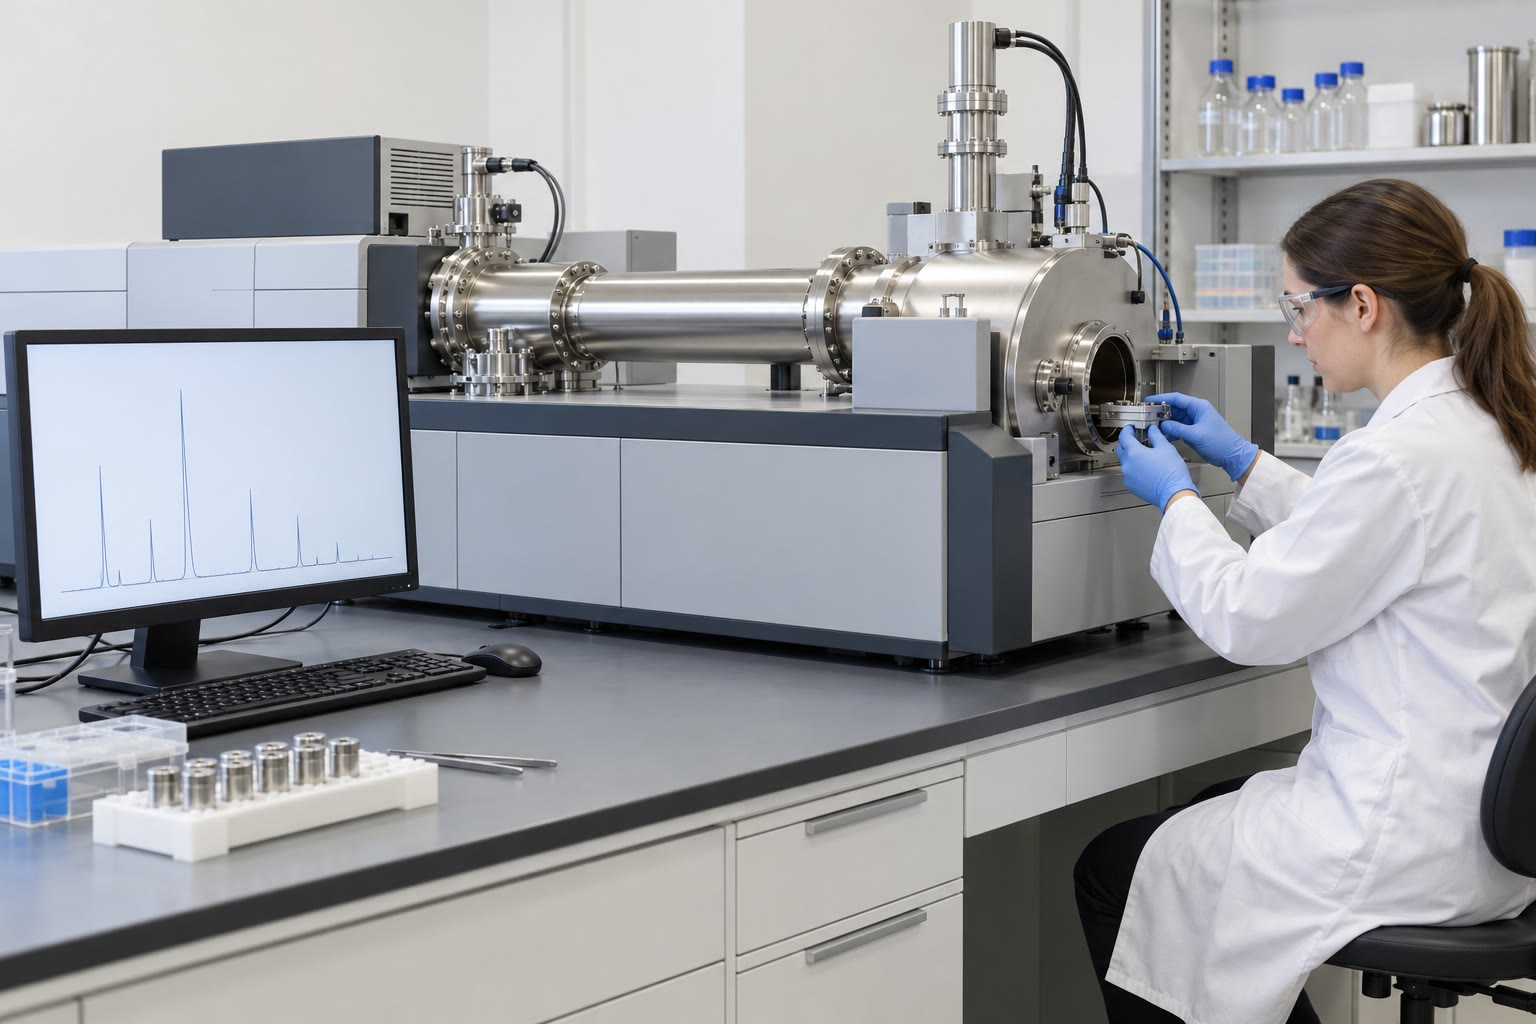
\includegraphics[width=0.66\linewidth]{images/book2/ai/g12-mass-spectrometer-lab.jpg}

{\small Een massaspectrometer in een laboratorium: er wordt een monster geladen aan de
kant van de bron. AI-illustratie.}
\end{omfigure}

De beginverhouding is ook een aanwijzing voor de herkomst van het magma. Rubidium
gaat bij voorkeur naar de smelt wanneer de mantel smelt, dus is het in de loop van de tijden
geconcentreerd in de \omterm{def:g12:continental-crust:continental-crust}{continentale korst}, die daardoor meer
strontium-87 heeft gemaakt: korstgesteenten hebben een hogere $^{87}\mathrm{Sr}/^{86}\mathrm{Sr}$
dan mantelgesteenten. Een magma uit gesmolten korst erft die hoge verhouding.
% ledger: tulane:radiometric

\section{De ouderdom van de Aarde}

Geen enkel gesteente op Aarde gaat terug tot het begin van de Aarde: het oudste bekende gesteente,
de gneis van Acasta, is 4.03 miljard jaar oud, en de oudste zirkoonkorrels 4.4
miljard. Het oppervlak is sindsdien gesmolten, geërodeerd en gerecycled. De datering
van de Aarde zelf komt van meteorieten, brokstukken van de kleine hemellichamen
die samen met de planeten ontstonden en waarvan sommige sindsdien gesloten systemen
zijn gebleven.
% ledger: bowring99:acasta, wilde01:zircon, usgs:age-earth (Book 1 row)

\begin{definition}[Ouderdom van de Aarde]\label{def:g12:age-of-the-earth:age}
De \emph{ouderdom van de Aarde}\index{ouderdom van de Aarde} is de tijd sinds de
Aarde ontstond door het samenklonteren van kleinere hemellichamen, bij de geboorte van het
zonnestelsel. Gemeten aan meteorieten door radiometrische datering is ze
\num{4.54} miljard jaar, tot op één procent nauwkeurig.
\end{definition}
% ledger: usgs:age-earth (Book 1 row)

In 1956 mat Clair Patterson de isotopen van lood in drie steenmeteorieten
en twee ijzermeteorieten. Twee isotopen van lood worden gemaakt door het
verval van uranium, lood-206 uit uranium-238 en lood-207 uit uranium-235,
terwijl lood-204 door geen enkel verval wordt gemaakt. Zoals bij strontium liggen de punten van meteorieten
die tegelijk zijn ontstaan op een rechte, wanneer
$^{207}\mathrm{Pb}/^{204}\mathrm{Pb}$ wordt uitgezet tegen
$^{206}\mathrm{Pb}/^{204}\mathrm{Pb}$. De ijzermeteoriet van Canyon Diablo, in
Arizona, bevat bijna geen uranium: zijn lood is sinds zijn ontstaan niet veranderd,
en markeert het onderste uiteinde van de rechte, het lood waarmee het zonnestelsel begon.
% ledger: patterson56:table, patterson56:constants, usgs:age-earth (Book 1 row: Canyon Diablo troilite)

\begin{omfigure}
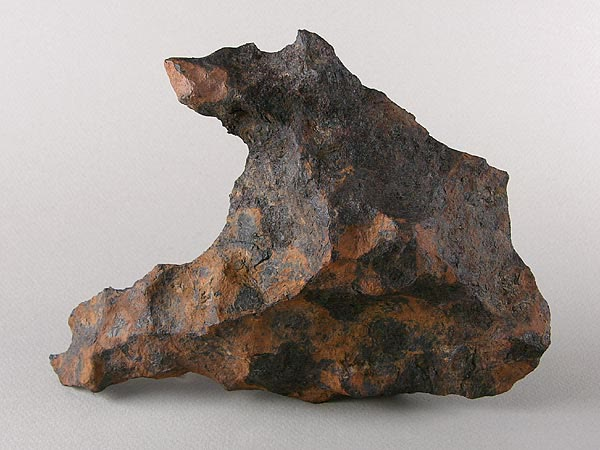
\includegraphics[height=4.2cm]{images/book2/g12-canyon-diablo-meteorite.jpg}

{\small Een brokstuk van de ijzermeteoriet van Canyon Diablo, \qty{2641}{g}.
Foto Geoffrey Notkin, CC~BY-SA~2.5 (Wikimedia Commons).}
\end{omfigure}
% ledger: photo:g12-canyon-diablo

Voor lood hangt de helling $m$ via beide uraniumisotopen van de ouderdom af; de
betrekking wordt hier aangenomen. Met de constanten die Patterson gebruikte, geldt
\[
  m = \frac{1}{137.8}\,\frac{e^{\lambda_{235}t}-1}{e^{\lambda_{238}t}-1},
  \qquad \lambda_{235} = \num{9.72e-10},\ \lambda_{238} = \num{1.537e-10}
  \text{ per jaar},
\]
wat geeft:
\begin{center}
\small
\begin{tabular}{|l|c|c|c|c|c|c|}
\hline
ouderdom (miljard jaar) & 4.40 & 4.45 & 4.50 & 4.55 & 4.60 & 4.65 \\
helling $m$ & 0.533 & 0.551 & 0.570 & 0.590 & 0.610 & 0.632 \\
\hline
\end{tabular}
\end{center}
% ledger: patterson56:constants
% values: pb_slope at 4.40-4.65 Ga (isochrons.py pb_slope)

\begin{omfigure}
\begin{tikzpicture}
\begin{axis}[omrecord, width=0.72\linewidth, height=6cm, xmin=0, xmax=56, ymin=0, ymax=40,
  xlabel={$^{206}\mathrm{Pb}/^{204}\mathrm{Pb}$}, ylabel={$^{207}\mathrm{Pb}/^{204}\mathrm{Pb}$}]
% computed in figdata/grade-12/isochrons.py; ledger: patterson56:table
\addplot[omDef, line width=0.9pt] table[x=x, y=y] {figdata/out/grade-12-isochrons-pbln.dat};
\addplot[omThm, only marks, mark=*, mark size=2pt] table[x=r206, y=r207, restrict expr to domain={\thisrow{idx}}{1:5}] {figdata/out/grade-12-isochrons-pbpb.dat};
\addplot[black, only marks, mark=o, mark size=2.6pt, line width=0.8pt] table[x=r206, y=r207, restrict expr to domain={\thisrow{idx}}{6:6}] {figdata/out/grade-12-isochrons-pbpb.dat};
\coordinate (nl) at (axis cs:50.28,34.86);
\coordinate (fc) at (axis cs:19.48,15.76);
\coordinate (cd) at (axis cs:9.5,10.36);
\coordinate (sed) at (axis cs:19.0,15.5);
\coordinate (sl) at (axis cs:30,25);
\end{axis}
\node[font=\scriptsize, anchor=north west] at ([xshift=2pt]nl) {Nuevo Laredo};
\node[font=\scriptsize, anchor=north west, align=left] at ([xshift=4pt, yshift=-2pt]fc) {Forest City, Modoc;\\oceaansediment (cirkel)};
\node[font=\scriptsize, anchor=north west, align=left] at ([xshift=3pt, yshift=-3pt]cd) {Canyon Diablo, Henbury (ijzer)};
\node[font=\scriptsize, text=omDef, anchor=south east] at (sl) {helling 0.603: ongeveer 4.6 miljard jaar};
\end{tikzpicture}

{\small De loodisochroon van Patterson: de vijf meteorieten liggen op één rechte, en
bijna ook het lood uit een modern oceaansediment, dat voor de Aarde staat.
Bron: Patterson (1956), tabel~1.}
\end{omfigure}
% values: pb_slope 0.6026, pb_age_Ga 4.58, sediment_residual -0.39 (isochrons.py)

Een rechte door de vijf punten heeft een helling van ongeveer 0.603, tussen
de hellingen voor 4.55 en 4.60 miljard jaar in de tabel. Pattersons eigen
resultaat, rekening houdend met de fouten van de metingen en van de
vervalconstanten, was 4.55 miljard jaar, op 0.07 na. Daarna mat hij lood uit een modern oceaansediment, dat
lood uit een grote massa van de aardkorst mengt: het ligt op dezelfde rechte. Het
lood van de Aarde is geëvolueerd zoals dat van de meteorieten, over dezelfde tijd: de
Aarde is even oud als zij.
% ledger: patterson56:table

Sindsdien hebben honderden metingen het bevestigd. Meteorieten geven ouderdommen
van 4.53 tot 4.58 miljard jaar, en de oudste vaste stoffen van het zonnestelsel,
kleine insluitsels rijk aan calcium en aluminium die in sommige meteorieten worden gevonden,
ontstonden \num{4567.30} miljoen jaar geleden, op 0.16 na. De Aarde ontstond
later uit zulk materiaal, en daarom is haar ouderdom, 4.54 miljard jaar, iets
kleiner dan die van hen.
% ledger: usgs:age-earth (Book 1 row), connelly12:cai

\section{Oefeningen}

\begin{exercise}[$\star$]\label{exo:g12:age-of-the-earth:1}
Geef het woord: (a) een mineraal waar sinds het begin van zijn klok geen moeder- of dochteratoom
in of uit is gegaan; (b) de rechte waarop mineralen van
één ouderdom en één bron liggen; (c) de tijd sinds de Aarde door
samenklonteren ontstond.
\end{exercise}

\begin{exercise}[$\star$]\label{exo:g12:age-of-the-earth:2}
Zet met de tabel van het graniet van Varden zijn vijf monsters op volgorde van
hun verhouding van rubidium-87 tot strontium-86, van de laagste af. Welk ervan
ligt het hoogst op de \omterm{def:g12:age-of-the-earth:isochron}{isochroon}, en waarom heeft het het meeste strontium-87 gemaakt?
\end{exercise}

\begin{exercise}[$\star$]\label{exo:g12:age-of-the-earth:3}
Bereken de halveringstijd van rubidium-87 uit zijn vervalconstante,
\num{1.3972e-11} per jaar. Hoeveel keer de \omterm{def:g12:age-of-the-earth:age}{ouderdom van de Aarde} is dat?
\end{exercise}

\begin{exercise}[$\star$]\label{exo:g12:age-of-the-earth:4}
Bereken $e^{\lambda t} - 1$ voor rubidium-87 voor $t = 310$ miljoen jaar en
$t = 480$ miljoen jaar.
\end{exercise}

\begin{exercise}[$\star$]\label{exo:g12:age-of-the-earth:5}
Zet de schattingen van Phillips, Holmes (1927), Joly, Kelvin
(1862) en Patterson op volgorde van datum. Hoeveel keer groter dan de bovengrens van de schatting van Joly
is de huidige \omterm{def:g12:age-of-the-earth:age}{ouderdom van de Aarde}?
\end{exercise}

\begin{exercise}[$\star\star$]\label{exo:g12:age-of-the-earth:6}
Een mineraal van het graniet van Varden (310 miljoen jaar, beginverhouding 0.7080)
heeft $^{87}\mathrm{Rb}/^{86}\mathrm{Sr} = 10.0$. Wat is zijn
$^{87}\mathrm{Sr}/^{86}\mathrm{Sr}$ vandaag? Wat was het toen het graniet
ontstond?
\end{exercise}

\begin{exercise}[$\star\star$]\label{exo:g12:age-of-the-earth:7}
Vier monsters van de schist van Varden geven $(x, y)$ = (0.90, 0.71806),
(2.60, 0.72950), (5.10, 0.74632) en (9.40, 0.77525), met $x =
{}^{87}\mathrm{Rb}/^{86}\mathrm{Sr}$ en $y = {}^{87}\mathrm{Sr}/^{86}\mathrm{Sr}$.
(1) Bereken uit het eerste en het laatste monster de helling en de ouderdom.
(2) Controleer dat de twee middelste monsters op dezelfde rechte liggen. (3) Is het
resultaat in overeenstemming met de 310 miljoen jaar van het graniet en het principe
van doorsnijding?
\end{exercise}

\begin{exercise}[$\star\star$]\label{exo:g12:age-of-the-earth:8}
Waarom geeft een gesteente waarin alle mineralen dezelfde verhouding van rubidium tot
strontium hebben, geen \omterm{def:g12:age-of-the-earth:isochron}{isochroon}? Waarom legt het biotiet in het graniet van Varden
de helling beter vast dan de andere mineralen?
\end{exercise}

\begin{exercise}[$\star\star$]\label{exo:g12:age-of-the-earth:9}
Lang nadat het graniet van Varden was ontstaan, liet een hete vloeistof zijn biotiet een deel
van zijn strontium-87 verliezen. (1) Waarheen verschuift zijn punt in het isochroondiagram?
(2) Welke ouderdom zouden het biotiet en het plagioklaas alleen dan geven: te oud of
te jong? (3) Hoe brengt de isochroonmethode het probleem aan het licht?
\end{exercise}

\begin{exercise}[$\star\star$]\label{exo:g12:age-of-the-earth:10}
(1) Hoeveel keer langer dan de 96 miljoen jaar van Kelvin is de \omterm{def:g12:age-of-the-earth:age}{ouderdom van de
Aarde}? (2) Joly nam aan dat de rivieren het zout in een constant tempo naar zee
voeren en dat er niets van de zee verlaat. Welke van deze aannames maakt zijn
ouderdom te kort als ze fout is, en waarom?
\end{exercise}

\begin{exercise}[$\star\star$]\label{exo:g12:age-of-the-earth:11}
Bereken met de waarden van Patterson voor Canyon Diablo (9.46, 10.34) en Nuevo Laredo
(50.28, 34.86) de helling van de rechte door de twee meteorieten,
en lees de ouderdom af uit de tabel van hellingen.
\end{exercise}

\begin{exercise}[$\star\star\star$]\label{exo:g12:age-of-the-earth:12}
Een basalt uit de streek van Varden, ook 310 miljoen jaar oud, heeft een
beginverhouding van 0.7035, tegen 0.7080 voor het graniet. (1) Welk gesteente komt eerder
uit gesmolten mantel, en welk uit gesmolten korst? (2) Leg uit
waarom, met wat je over rubidium weet. (3) Kunnen de twee uit
één magma zijn gekristalliseerd?
\end{exercise}

\begin{exercise}[$\star\star\star$]\label{exo:g12:age-of-the-earth:13}
(1) Welk deel van het rubidium-87 dat aanwezig was toen de Aarde ontstond, is er
vandaag nog? En van het uranium-238 (halveringstijd 4.47 miljard jaar)? (2) Wat zou
de helling zijn van een rubidium-strontiumisochroon voor een gesteente van één miljoen jaar
oud? Waarom is rubidium-strontium een slechte klok voor jonge gesteenten?
\end{exercise}

\begin{exercise}[$\star\star\star$]\label{exo:g12:age-of-the-earth:14}
De rechte door de vijf meteorieten van Patterson is $y = 4.438 + 0.6026\,x$.
(1) Welke $^{207}\mathrm{Pb}/^{204}\mathrm{Pb}$ voorspelt ze voor het
oceaansediment, bij $x = 19.0$? Patterson mat 15.5: hoeveel procent verschillen ze?
(2) Welke ouderdom geeft de helling 0.6026 volgens de tabel? Vergelijk met
Pattersons $4.55 \pm 0.07$ miljard jaar.
\end{exercise}

\begin{exercise}[$\star\star\star$]\label{exo:g12:age-of-the-earth:15}
Kelvin nam aan dat alle warmte die de Aarde verliest, vandaag \qty{46.7}{TW}, opgeslagen
warmte is. (1) Radioactiviteit vult er ongeveer \qty{24.4}{TW} van aan. Hoeveel
verlengt dat alleen al de tijd om een gegeven voorraad warmte te verliezen?
(2) Is dat, vertrekkend van 96 miljoen jaar, genoeg om de ware ouderdom te bereiken?
(3) Wat miste Kelvin dat zwaarder weegt?
\end{exercise}

\begin{problem}[{Weekendprobleem --- het graniet van Varden dateren}]
\label{pb:g12:age-of-the-earth:1}
% exercise data from figdata/grade-12/isochrons.py; ledger: villa22:rb87, tulane:radiometric, ics:base.Carboniferous, ics:base.Permian
Het graniet van de Varden Hills, de verzonnen streek van de reeks, doorsnijdt de
schist eromheen. Een laboratorium mat vijf van zijn monsters (voorbeeld hierboven):
plagioklaas (0.35, 0.70952), hoornblende (1.20, 0.71321), heel gesteente (3.10,
0.72146), K-veldspaat (6.40, 0.73578) en biotiet (24.0, 0.81218), elk als
$(^{87}\mathrm{Rb}/^{86}\mathrm{Sr},\ ^{87}\mathrm{Sr}/^{86}\mathrm{Sr})$. De
vervalconstante van rubidium-87 is \num{1.3972e-11} per jaar.

\medskip
\noindent\textbf{Deel I --- De monsters.}
\begin{enumerate}
  \item Welk monster is het rijkst aan rubidium ten opzichte van strontium?
  \item Waarom begonnen alle mineralen met dezelfde
        $^{87}\mathrm{Sr}/^{86}\mathrm{Sr}$?
  \item Waarom worden de verhoudingen op strontium-86 betrokken?
  \item Welke van de drie isotopen is toegenomen sinds het graniet ontstond, en
        waarom?
  \item Hoe zagen de vijf punten eruit in het diagram toen het graniet
        net was ontstaan?
\end{enumerate}

\medskip
\noindent\textbf{Deel II --- De isochroon.}
\begin{enumerate}[resume]
  \item Bereken de helling door het plagioklaas en het biotiet.
  \item Bereken de helling door het plagioklaas en het hele gesteente.
  \item Vergelijk de twee hellingen. Welke is betrouwbaarder, en waarom?
  \item Bepaal waar de rechte van vraag 6 de verticale as snijdt.
  \item Controleer dat het K-veldspaat op die rechte ligt.
\end{enumerate}

\medskip
\noindent\textbf{Deel III --- De helling en de ouderdom.}
\begin{enumerate}[resume]
  \item Schrijf de betrekking tussen de helling en $e^{\lambda t}$.
  \item Bereken $\lambda t$.
  \item Bereken de ouderdom $t$.
  \item De schist is gedateerd op 480 miljoen jaar. Is de volgorde van de
        twee ouderdommen wat de terreinverhoudingen vereisen?
  \item Het Carboon loopt van 358.9 tot 298.9 miljoen jaar geleden. In
        welke periode ontstond het graniet?
\end{enumerate}

\medskip
\noindent\textbf{Deel IV --- De beginverhouding en de bron.}
\begin{enumerate}[resume]
  \item Wat stelt het snijpunt, 0.7080, voor?
  \item Een basalt uit de streek ontstond met een verhouding van 0.7035. Welk gesteente
        heeft de hoogste beginverhouding?
  \item Waarom hebben korstgesteenten hogere verhoudingen dan de mantel?
  \item Wat doet de beginverhouding van het graniet vermoeden over het gesteente dat
        smolt om het te maken?
  \item Vat samen: hoe oud is het graniet van Varden?
\end{enumerate}
\end{problem}
